\section{Методы решения задачи}

В данной работе была написана программная реализация метода максимального правдоподобия, которая описана в приложении А. Также был написан программный комплекс, представляющий собой веб-сервис по работе с методом максимального правдоподобия, описан в приложении Б.


\subsection{Признаковые пространства}

Сформируем признаковые пространства для моделей, основанных как на Пуассоновской регрессии, так и на геометрической регрессии:

\begin{enumerate}[label=\arabic*.]
    \item $features_1:$ (кривизна);
    \item $features_2:$ (кривизна, профиль пути);
    \item $features_3:$ (кривизна, профиль пути $\cdot$ макс. число вагонов в сходе);
    \item $features_4:$ (кривизна, $1 - \frac{\text{макс. число вагонов в сходе}}{\text{общее кол-во вагонов}}$);
    \item $features_5:$ (кривизна, профиль пути, скорость $\cdot$ загрузка);
    \item $features_6:$ (кривизна, профиль пути, скорость $\cdot$ загрузка,\\ $1 - \frac{\text{макс. число вагонов в сходе}}{\text{общее кол-во вагонов}}$);
    \item $features_7:$ (кривизна, скорость $\cdot$ загрузка, $1 - \frac{\text{макс. число вагонов в сходе}}{\text{общее кол-во вагонов}}$);
    \item $features_8:$ (скорость $\cdot$ загрузка, $1 - \frac{\text{макс. число вагонов в сходе}}{\text{общее кол-во вагонов}}$).
    \newline
\end{enumerate}
Также в каждый набор признаков добавим новый признак $Intercept$, реализация которого всегда равна единице. Данный признак необходим для появления свободного члена $\theta_0$ в результате скалярного произведения: $\left\langle \theta, x\right\rangle = \theta_0 + \theta_1 x_1 + \theta_2 x_2 + \ldots + \theta_n x_n$, где $n+1$ -- размерность соответствующего признакового пространства.

Были добавлены новые признаки, такие как: профиль пути $\cdot$ макс. число вагонов в сходе, $1 - \frac{\text{макс. число вагонов в сходе}}{\text{общее кол-во вагонов}}$, скорость $\cdot$ загрузка. Вычислим коэффициенты корреляции новых признаков с целевой целевым признаком количество сошедших вагонов, а также вычислим коэффициенты корреляции между самими признаками (для удобства чтения таблицы сделаем соответствующие переименование признаков: target, $f_1$, $f_2$, $f_2$, $f_3$):


\begin{table}[H]
    \captionof{table}{Корреляция целевого признака с введеными}
    \label{tab:corr_new_features}
    \begin{tabular}{|l|c|c|c|c|}
        \hline
        & target & $f_1$ & $f_2$ & $f_3$ \\ \hline
        target & 1.0       & 0.101375  & -0.286535 & 0.198847  \\ \hline
        $f_1$  & 0.101375  & 1.0       & -0.086693 & -0.228508 \\ \hline
        $f_2$  & -0.286535 & -0.086693 & 1.0       & -0.124420 \\ \hline
        $f_3$  & 0.198847  & -0.228508 & -0.124420 & 1.0       \\ \hline
    \end{tabular}
\end{table}


Из таблицы видно, что признаки $f_1$ и $f_3$ имеют значительную величину корреляции между собой. При этом признак $f_2$ слабо коррелирует как с $f_1$, так и с $f_3$. Из этого следует, что в один набор признаков нежелательно включать $f_1$ и $f_3$ вместе.

Также можно заметить, что признак $f_2$ сильно коррелирует с целевым признаком.





\subsection{Пуассоновская регрессия}

Предположим, что количество сошедших вагонов имеет Пуассоновское распределение. Тогда функция вероятности $p(k) = \dfrac{\lambda^k}{k!}e^{-\lambda}$. Пусть плотность потока событий $\lambda = \lambda(\theta, x)$, где $\theta$ -- вектор параметров, $x$ -- вектор, описывающий объект. Выберем набор функций $\lambda$, параметризованных по $\theta$:
\begin{enumerate}[label=\arabic*.]
    \item $\lambda_1(\theta, x) = e^{\left\langle \theta, x\right\rangle}$;
    \item $\lambda_2(\theta, x) = e^{-[\left\langle \theta, x\right\rangle]^2}$;
    \item $\lambda_3(\theta, x) = \sqrt{|5^2 - (\left\langle \theta, x\right\rangle - 5)^2|} + 1$;
    \item $\lambda_4(\theta, x) = (\left\langle \theta, x\right\rangle - 1)^2$;
    \item $\lambda_5(\theta, x) = \frac{1}{1 + (\left\langle \theta, x\right\rangle)^2}$;
    \item $\lambda_6(\theta, x) = \left\langle \theta, x\right\rangle (\frac{\pi}{2} + \arctan(\left\langle \theta, x\right\rangle)) + 1$;
    \item $\lambda_7(\theta, x) = \log(1 + (\left\langle \theta, x\right\rangle)^2) + 1$.
\end{enumerate}

В качестве оптимизационного метода был выбран топологический метод глобальной оптимизации SHGO (Simplicial Homology Global Optimisation), реализованный в модуле scipy.optimize. В качестве граничного множества для искомых параметров был взят гиперкуб со стороной $2000$ и центром в начале координат (т.е$. -1000 \leq \theta_i \leq 1000~~i = \overline{0,n}$, где $n$ -- размерность соответствующего признакового пространства).

Ранее была получена функция логарифмического правдоподобия: $l(\theta, x) = \sum\limits_{i=1}^{N} \left( -\lambda(\theta, x) + y_i \ln(\lambda(\theta, x)) - \ln(y_i!) \right)$. Программно реализовав данную функцию и запустив метод fit\_all у объекта класса MLM, были получены следующие результаты:

\subfile{poisson_table}

%Заметим, что для моделей с $\lambda=\lambda_2$ оценки параметра $\hat\theta$ получились тривиальными, то есть все компоненты вектора $\hat\theta$ получились равными нулю. Также для моделей с $\lambda=\lambda_5$ оценка $\hat\theta$ тривиальная для всех признаковых пространств. Также можно заметить, что для моделей с $\lambda=\lambda_3$ некоторые оценки также тривиальны.

%Заметим также, что для тривиальных моделей, соответствующих одному признаковому пространству, критерии Акаике совпадают, например, для $(features_7, \lambda_2) AIC_c = 574.21$, для $(features_7, \lambda_3) AIC_c = 574.21$, для $(features_7, \lambda_5) AIC_c = 574.21$.


Общий диапазон значений критерия Акаике для всех моделей: $AIC_c \in [356.87, 567.74]$.


Наилучшее значение по показателям качества получилось для модели $(features_7, \lambda_1)$. Таким образом, в моделях Пуассоновской регрессии показатель качества по критерию Акаике для наилучшей модели равняется $356.87$.



Будем считать модель тривиальной, если ее признаковое пространство имеет размерность, равную единице. При этом для всех наблюдений данное свойство имеет постоянное значение. Вычислим значение критерия Акаике для тривиальной модели. В качестве исходных наблюдений возьмем такой же набор, как в модели, соответствующей $(features_7, \lambda_1)$. Проведя вычисления, было получено, что $AIC_{c, trivial} = 551.27$. Найдем отношение $AIC_c$, соответствующей наилучшей модели, к $AIC_{c, trivial}$. По данному отношению можно считать качество модели, которое может изменяться от нуля до единицы. При этом чем ближе значение к нулю, тем больше качество модели. Рассчитав значение данного отношения, получим, что $\dfrac{AIC_c}{AIC_{c, trivial}} = 0.54$.



%Учитывая, что для каждого признакового пространства нашлась хотя бы одна тривиальная модель модель, оставшиеся нетривиальные модели можно сравнивать с ними в рамках одного признакового пространства.

%\begin{table}[H]
%    \resizebox{\textwidth}{!}{
%    \begin{tabular}{|l|c|c|c|c|c|c|c|c|}
%        \hline
%        & $features_1$ & $features_2$ & $features_3$ & $features_4$ & $features_5$ & $features_6$ & $features_7$ & $features_8$ \\ \hline
%        $AIC_{c,best}$ & $516.56$ & $477.09$ & $453.11$ & $444.77$ & $446.29$ & $425.77$ & $400.13$ & $410.65$ \\ \hline
%        $AIC_{c,trivial}$ & $617.6$ & $606.39$ & $598.47$ & $611.95$ & $586.35$ & $575.39$ & $574.21$ & $575.39$ \\ \hline
%        $\frac{AIC_{c,best}}{AIC_{c,trivial}}$ & $0.83$ & $0.79$ & $0.75$ & $0.73$ & $0.76$ & $0.74$ & $0.69$ & $0.7$ \\ \hline
%        Мощность выборки & 46 & 41 & 37 & 42 & 42 & 37 & 35 & 37 \\ \hline
%        $\lambda_{i, best}$ & $\lambda_4$ & $\lambda_3$ & $\lambda_6$ & $\lambda_6$ & $\lambda_6$ & $\lambda_6$ & $\lambda_1$ & $\lambda_1$ \\ \hline
%    \end{tabular}
%    }
%\end{table}
%\captionof{table}{Сравнение лучших моделей Пуассоновской регрессии с тривиальными}
%\label{tab:poisson_comp}

%\begin{wrapfigure}{r}{0.35\linewidth} 
%    \vspace{1ex}
%    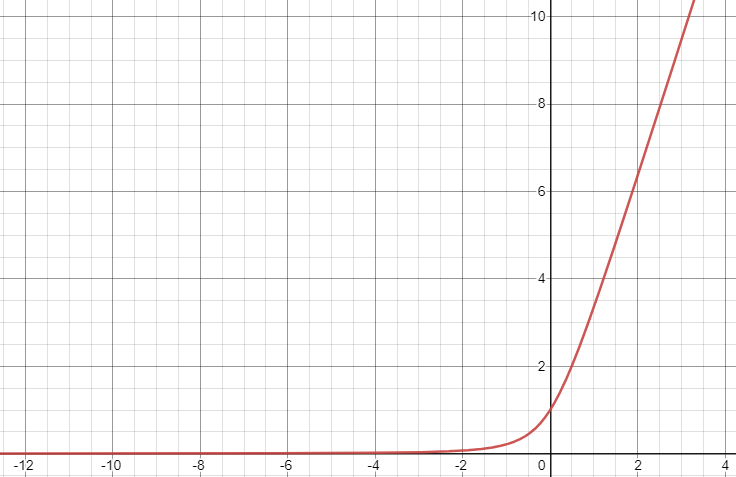
\includegraphics[width=\linewidth]{src/img/rounded_relu.png}
%    \caption{Сглаженная ReLU}
%    \label{fig:rounded_relu}
%\end{wrapfigure}

%В 4 из 8 признаковых пространств функция $\lambda_6$ оказалась наилучшей среди других по значению критерия Акаике. Данная функция эквивалентна функции $f(x) = x \left( \dfrac{\pi}{2} + \arctan(x) \right) + 1$. По своей структуре данная функция напоминает функцию $ReLU(x) = \begin{cases}
%    x, &\text{если $x > 0$,}\\
%    0, &\text{иначе.}
%\end{cases}$, при этом $f(x)$, очевидно, также имеет 2 асимптоты: $y=\pi x$, $y=0$. В отличие от классической функции ReLU она является более гладкой, имеет непрерывную производную во всех точках.


\subsection{Геометрическая регрессия}

Предположим, что количество сошедших вагонов имеет геометрическое распределение. Тогда функция вероятности $p(n) = (1-p)^n p$. Пусть вероятность успеха в серии испытаний Бернулли $p = p(\theta, x)$, где $\theta$ -- вектор параметров, $x$ -- вектор, описывающий объект. Выберем набор функций $p$, параметризованных по $\theta$:
\begin{enumerate}[label=\arabic*.]
    \item $p_1(\theta, x) = e^{\left\langle \theta, x\right\rangle}$;
    \item $p_2(\theta, x) = e^{-[\left\langle \theta, x\right\rangle]^2}$;
    \item $p_3(\theta, x) = \frac{1}{1+e^{-\left\langle \theta, x\right\rangle}}$;
    \item $p_4(\theta, x) = \frac{1}{1 + [\left\langle \theta, x\right\rangle]^2}$;
    \item $p_5(\theta, x) = \left\langle \theta, x\right\rangle (\frac{\pi}{2} + \arctan(\left\langle \theta, x\right\rangle)) + 1$.
\end{enumerate}

Метод SHGO, использованный при оптимизации в Пуассоновской регрессии, оказался не успешным для геометрической регрессии и данного набора данных. Ни для одной модели геометрической регрессии не удалось найти оптимальную точку. Вероятно, это связано со сложным видом оптимизационной функции в признаковых пространствах. По этой причине были использованы другие методы глобальной оптимизации (Dual Annealing, Differential Evolution, Basin-hopping), также реализованные в модуле scipy.optimize.

Наилучшие результаты были получены с помощью метода Dual Annealing (алгоритм имитации обжига). В качестве граничного множества для искомых параметров был взят гиперкуб со стороной  $2000$ и центром в начале координат (т.е$. -1000 \leq \theta_i \leq 1000~~i = \overline{0,n}$, где $n$ -- размерность соответствующего признакового пространства).

Ранее была получена функция логарифмического правдоподобия: $l = \sum\limits_{i = 1}^N ( y_i \ln(1 - p(\theta, x_i)) + \ln(p(\theta, x_i)) )$. Программно реализовав данную функцию и запустив метод fit\_all у объекта класса MLM, были получены следующие результаты:

\clearpage
\subfile{geometry_table}


Общий диапазон значений критерия Акаике для всех моделей: $AIC_c \in [153.65, 918.43]$.


Наилучшее значение по показателям качества получилось для модели $(features_7, p_4)$. Таким образом, в моделях геометрической регрессии показатель качества по критерию Акаике для наилучшей модели равняется $153.65$.


Так же как и для Пуассоновской регрессии вычислим отношение значения критерия Акаике лучшей модели к соответствующей ей тривиальной модели: $\dfrac{AIC_c}{AIC_{c, trivial}} = \dfrac{153.65}{249.89} = 0.61$.



%Построим тривиальные модели для каждого признакового пространства. Для сравнения с оставшимися моделями.

%\begin{table}[H]
%    \resizebox{\textwidth}{!}{
%        \begin{tabular}{|l|c|c|c|c|c|c|c|c|}
%            \hline
%            & $features_1$ & $features_2$ & $features_3$ & $features_4$ & $features_5$ & $features_6$ & $features_7$ & $features_8$ \\ \hline
%            $AIC_{c,best}$ & $200.3$ & $178.59$ & $165.23$ & $174.73$ & $168.97$ & $160.83$ & $153.79$ & $155.27$ \\ \hline
%            $AIC_{c,trivial}$ & $241.34$ & $234.01$ & $228.53$ & $238.15$ & $227.05$ & $219.97$ & $220.01$ & $219.97$ \\ \hline
%            $\frac{AIC_{c,best}}{AIC_{c,trivial}}$ & $0.83$ & $0.76$ & $0.72$ & $0.73$ & $0.74$ & $0.73$ & $0.69$ & $0.7$ \\ \hline
%            Мощность выборки & 46 & 41 & 37 & 42 & 42 & 37 & 35 & 37 \\ \hline
%            $p_{i, best}$ & $p_5$ & $p_4$ & $p_4$ & $p_4$ & $p_4$ & $p_4$ & $p_4$ & $p_4$ \\ \hline
%        \end{tabular}
%    }
%\end{table}
%\captionof{table}{Сравнение лучших моделей геометрической регрессии с тривиальными}
%\label{tab:geom_comp}

Следует отметить, что большая часть полученных значений критерия Акаике в геометрической регрессии меньше, чем полученные значения критерия Акаике в Пуассоновской регрессии, что говорит о том, что модели геометрической регрессии для данной задачи являются более предпочтительными по сравнению с моделями Пуассоновской регрессии.
%Также отношения значения критерия Акаике наилучшей модели к соответствующей тривиальной модели для двух типов регрессий отличаются более чем на порядок.




